\chapter{Optical Activity in Hyper-Rayleigh Scattering}\label{sec:results:HRS}

\color{red}
Additional information to include
\begin{itemize}
    \item Precise laser specifications ($\SI{18.9}{\milli\watt}\pm\SI{0.1}{\milli\watt}$ average power for all wavelengths)
    \item Ag spherical nanoparticle colloidal solution reference, demonstrating depolarisation effects of the helix anisotropy.
\end{itemize}
\color{black}

\section{Introduction}

\begin{figure}[htb!]	
    \centering	
    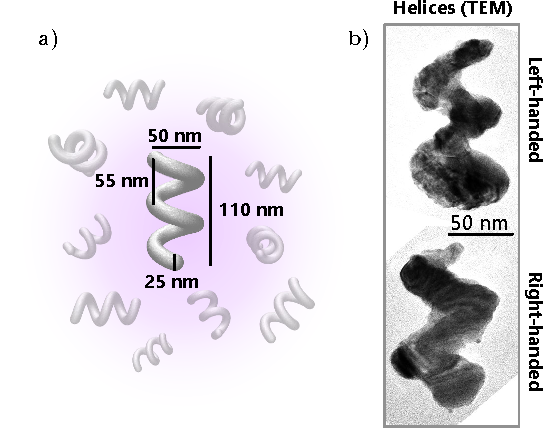
\includegraphics[scale=1]{./figures/results/HRS/sample_schematic.pdf}
    \caption{\label{fig:results:HRS:sample_schematic}
    \textbf{a)} Dimensions (center-to-center) of the nanohelices isotropically dispersed in water. Helix height is $\SI{110}{\nano\m}$, loop diameter is $\SI{50}{\nano\m}$, loop pitch is $\SI{55}{\nano\m}$, and wire-diameter is $\SI{25}{\nano\m}$. \textbf{b)} Transmission Electron Microscopy (TEM) images of left- and right-handed helices. }	
\end{figure}

\begin{figure}[htb!]	
    \centering	
    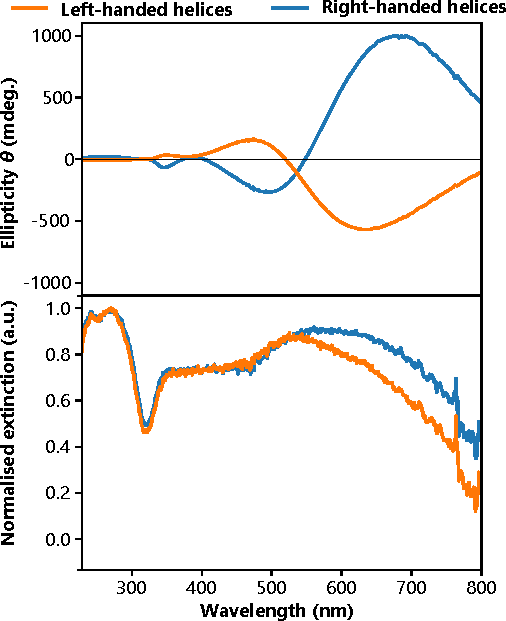
\includegraphics[scale=1]{./figures/results/HRS/linear_data.pdf}
    \caption{\label{fig:results:HRS:linear_data}
    Linear characterization of the nanohelix solutions. Left: ellipticity spectra, as measured with a CD spectrometer, through a $\SI{1}{\centi\m}$ path length filled with left- and right-handed nanohelix suspensions. Right: corresponding normalized extinction spectra from the left- and right-handed nanohelix suspensions. Extinction is obtained from the transmission spectrum and describes both absorption and scattering losses.}	
\end{figure}

\section{Results}

\begin{figure}[htb!]	
    \centering	
    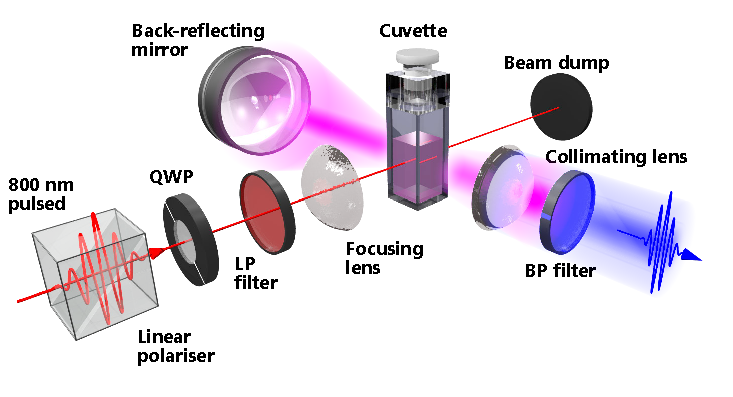
\includegraphics[scale=1]{./figures/results/HRS/experiment_schematic.pdf}
    \caption{\label{fig:results:HRS:experiment_schematic}
    Schematic diagram of the hyper-Rayleigh scattering circular dichroism experimental setup. QWP: quarter wave-plate; LP filter: long-pass filter; BP filter: band pass filter. }	
\end{figure}

\begin{figure}[htb!]	
    \centering	
    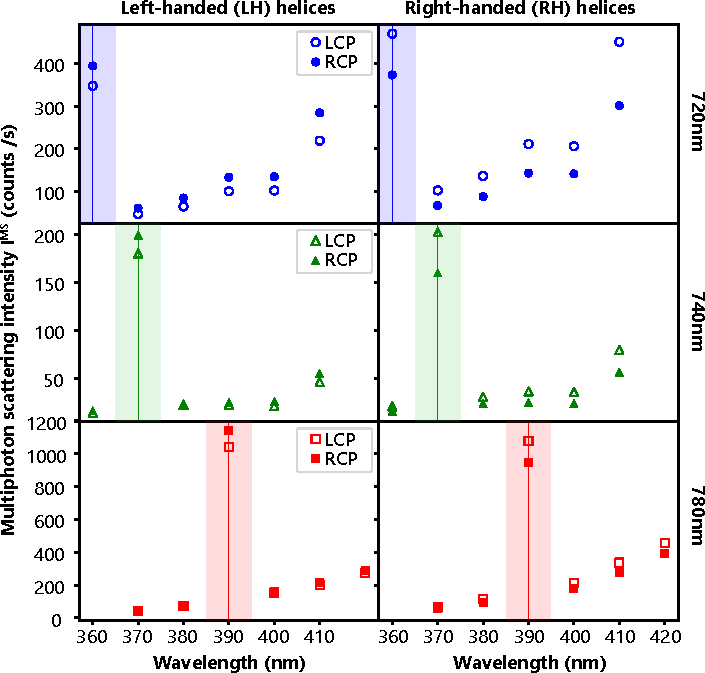
\includegraphics[scale=1]{./figures/results/HRS/hrs_data.pdf}
    \caption{\label{fig:results:HRS:hrs_data}
    Multi-photon scattering spectra for left- and right-handed helices, under LCP and RCP illumination. Results obtained for fundamental wavelengths of $\SI{720}{\nano\m}$, $\SI{740}{\nano\m}$ and $\SI{780}{\nano\m}$ are shown in blue, green, and red, respectively. Vertical colored lines mark the HRS (second-harmonic) wavelength, demonstrating clear peaks above the multiphoton luminescence background. The HRS unambiguously follows variations of the fundamental. }	
\end{figure}

\begin{figure}[htb!]	
    \centering	
    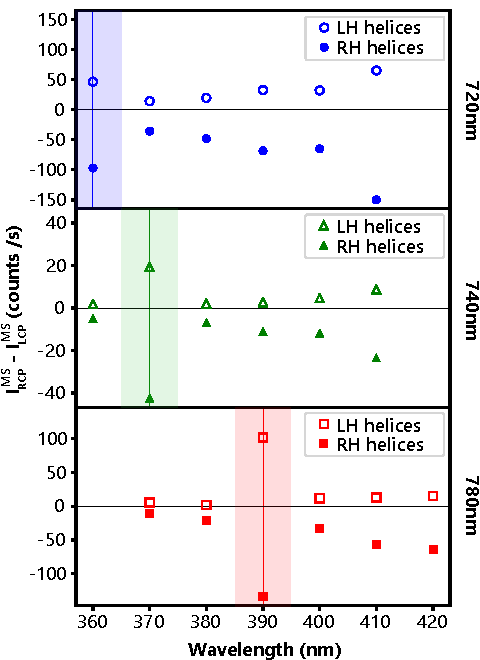
\includegraphics[scale=1]{./figures/results/HRS/hrs_cd_data.pdf}
    \caption{\label{fig:results:HRS:hrs_cd_data}
    Circular difference ($I_{RCP}^{MS}-I_{LCP}^{MS}$) in multiphoton scattering intensity, for both left-handed (LH) and right-handed (RH) nanohelix suspensions. Again, pump wavelengths of $\SI{720}{\nano\m}$, $\SI{740}{\nano\m}$ and $\SI{780}{\nano\m}$ are shown in blue, green, and red, respectively, and vertical coloured lines mark the HRS (second-harmonic) wavelength. The HRS circular difference clearly reverses between nanohelix enantiomorphs.}	
\end{figure}

\begin{table}[tbp]
    \begin{tabular}{llll}
    \firsthline
                                                                & \textbf{\begin{tabular}[c]{@{}l@{}}Fundamental \\ wavelength (nm)\end{tabular}} & \textbf{\begin{tabular}[c]{@{}l@{}}Linear \\ ellipticity (mdeg.)\end{tabular}} & \textbf{\begin{tabular}[c]{@{}l@{}}HRS \\ ellipticity (mdeg.)\end{tabular}} \\ 
    \hline
    \multirow{3}{*}{\begin{tabular}[c]{@{}l@{}}Right-handed \\ helices\end{tabular}}  & 720                                                                    & 920                                                                   & -3299                                                              \\
                                                                & 740                                                                    & 803                                                                   & -3356                                                              \\
                                                                & 780                                                                    & 569                                                                   & -1890                                                              \\ 
    \hline
    \multirow{3}{*}{\begin{tabular}[c]{@{}l@{}}Left-handed \\ helices\end{tabular}}& 720                                                                    & -370                                                                  & 1811                                                               \\
                                                                & 740                                                                    & -293                                                                  & 1455                                                               \\
                                                                & 780                                                                    & -164                                                                  & 1334                                                               \\ 
    \lasthline
    \end{tabular}
    \caption{Linear and HRS ellipticities for left- and right-handed nanohelix suspensions. Values are given at the three fundamental wavelengths used in the HRS experiments.}
    \label{table:HRS:ellipticity}
\end{table}

\begin{figure}[htb!]	
    \centering	
    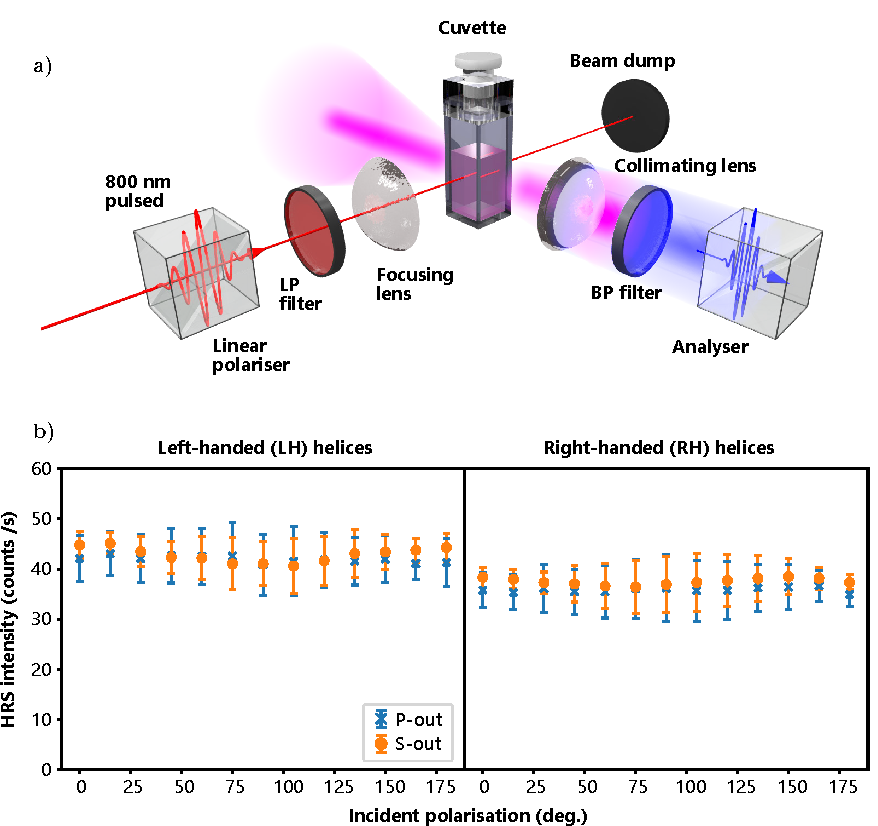
\includegraphics[scale=1]{./figures/results/HRS/hrs_linpol_data.pdf}
    \caption{\label{fig:results:HRS:hrs_linpol_data}
    The nanohelices are isotropically suspended in water. \textbf{a)} Schematic of the setup used to measure hyper-Rayleigh scattering of linearly polarised incident light. \textbf{b)} P-polarised (blue crosses) and S-polarised (orange dots) HRS intensity at $\SI{360}{\nano\m}$, as the polarization of $\SI{720}{\nano\m}$ incident light is rotated. Both left-handed (LH) and right-handed (RH) nanohelix suspensions exhibit no variation outside of experimental uncertainty, demonstrating a clear isotropic arrangement of helices within the liquid suspension.}	
\end{figure}

\section{Discussion}
\section{Conclusions}